\chapter{Background}

\section{Remote Sensing}
Remote sensing (RS) is commonly defined as the acquisition of information about an object through sensors without direct physical contact. This information is obtained by detecting and measuring the modifications the object induces in its surrounding fields, which may include electromagnetic, acoustic, or potential fields \cite{book_Physics_Techniques_RS}.

RS is a relatively recent scientific discipline characterized by its strong interdisciplinary nature. It draws upon a wide spectrum of fields, requiring practitioners to develop a broad foundational understanding of both natural and applied sciences. Effective research in remote sensing often involves collaboration with specialists in electromagnetic theory, spectroscopy, applied physics, geology, atmospheric sciences, oceanography, electrical engineering, and optical engineering \cite{book_Physics_Techniques_RS}.

Remote observations require an interaction of energy between the target and the sensor. In the case of passive sensors, the detected energy originates from external or natural sources, such as solar radiation reflected by the Earth's surface or thermal radiation emitted by the object itself. A prominent example is the \textit{Landsat} program \footnote{https://landsat.gsfc.nasa.gov/}, which represents the longest continuously operating Earth observation mission. Over several decades, Landsat has generated a continuous global record, contributing significantly to environmental monitoring and Earth system science.

By contrast, active sensors generate their own energy pulses to illuminate the target and subsequently measure the portion of the signal that is reflected or backscattered. This capability allows them to operate independently of solar illumination and under a wide range of environmental conditions, including day or night and, in the case of microwave systems, through cloud cover and adverse weather \cite{RS_platforms_survey}. The most widely used active sensing technologies are Radar (Radio Detection and Ranging), which transmits and receives microwave radiation, and LiDAR (Light Detection and Ranging), which employs laser pulses in the optical domain. Both systems record the properties of the reflected signals to extract information about the target.

The term \textit{Remote Sensing} was introduced in the early 1960s to denote techniques for observing the Earth from a distance, with particular reference to aerial photography, which represented the predominant sensing technology at that time \cite{book_Satellite_RS}.

With the advent of satellites, global and synoptic observations of Earth and other planetary environments have become possible. Earth-orbiting sensors provide essential data on atmospheric dynamics, cloud distribution, vegetation cover, and its seasonal variability. Their long-term operation and repetitive coverage enable the monitoring of rapidly changing processes, such as polar ice dynamics and tropical deforestation. Beyond Earth, planetary missions (orbiters, flybys, landers, and rovers) have extended similar observations to all major planets in the solar system. To date, every planet has been visited at least once \cite{book_Physics_Techniques_RS}.
% \newpage

The origins of remote sensing date back to the invention of photography in 1839, which soon after was applied to topographic mapping. By the mid-19th century, aerial photographs were obtained from balloons, followed later by kites, pigeons, and eventually airplanes—the latter marking a decisive step with Wilbur Wright's first aerial photographs in 1909. Aerial photography became essential during World War I and advanced further in the 1930s-1940s with the introduction of color and infrared-sensitive films, widely used during World War II for reconnaissance and camouflage detection \cite{book_Physics_Techniques_RS,book_Satellite_RS}.

\begin{figure}[H]
  \centering
  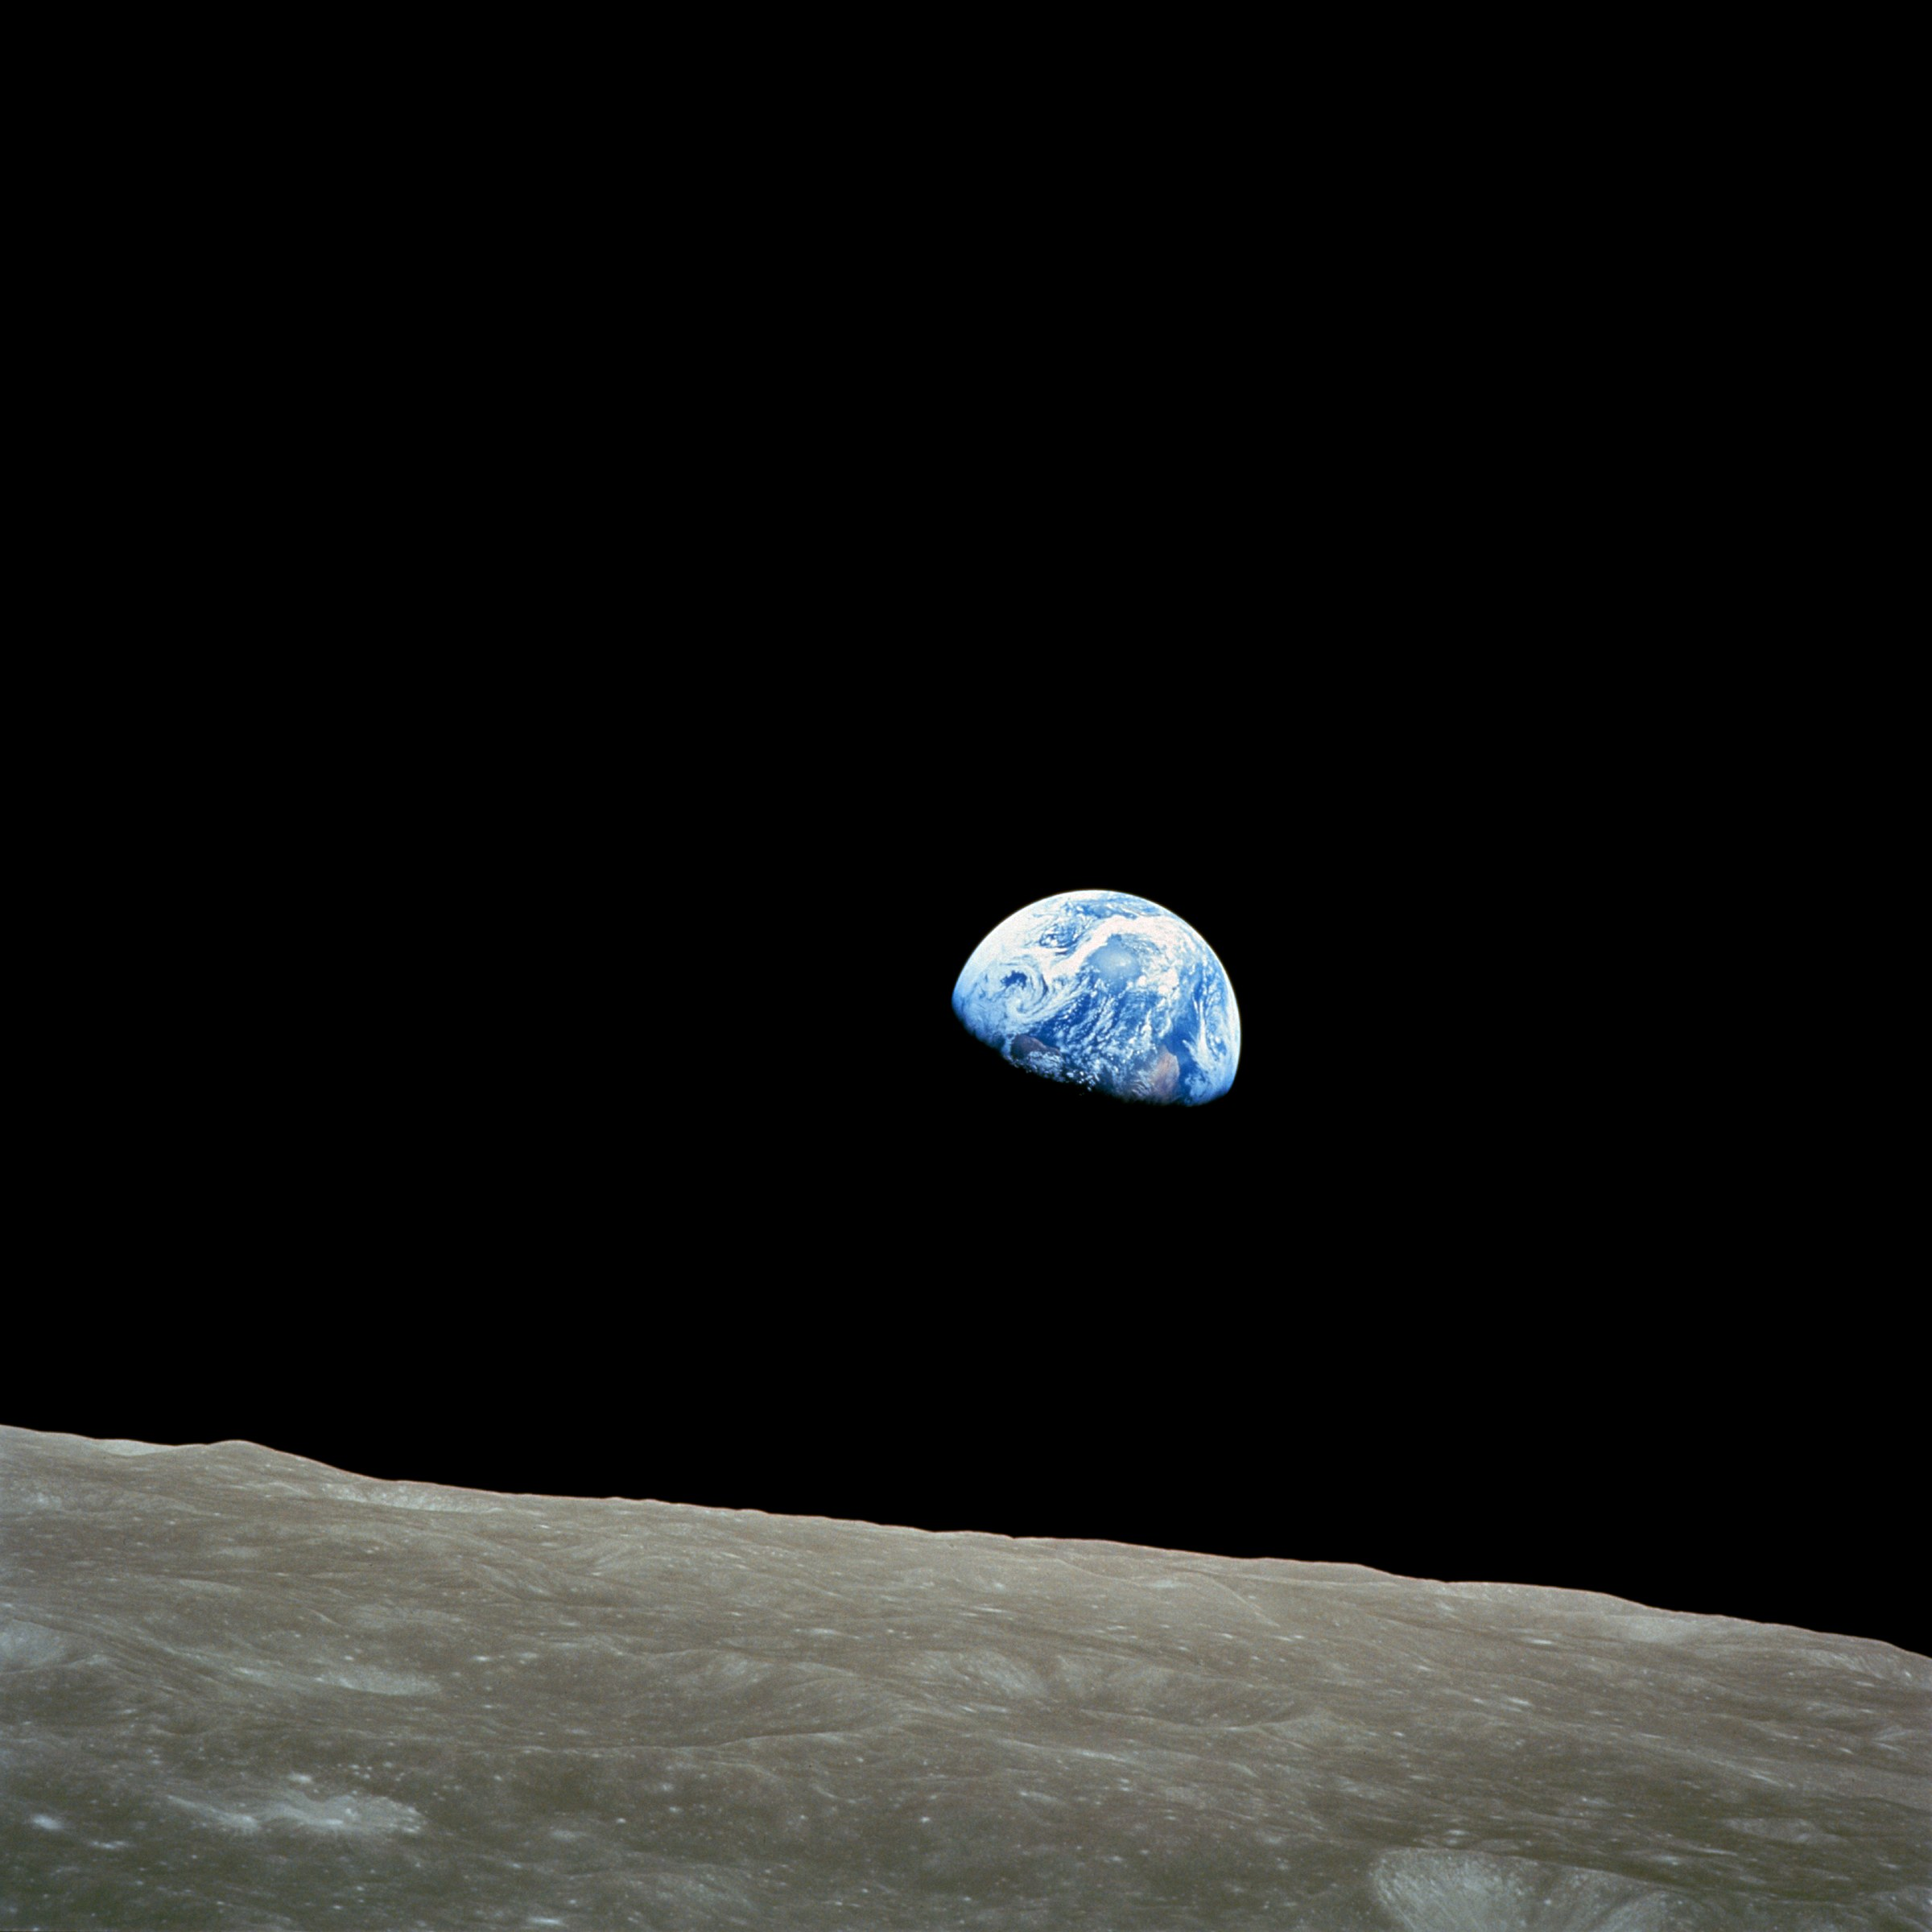
\includegraphics[width=0.95\textwidth]{img/earthrise.jpg}
  \caption{The iconic “Earthrise” photograph taken by astronaut William Anders during the Apollo 8 mission in 1968. Source: NASA.}
  \label{fig:earthrise}
\end{figure}

The postwar decades brought rapid technological progress with the development of radar and synthetic aperture radar (SAR), enabling high-resolution imaging independent of daylight or weather. Early rocket experiments in the late 1940s foreshadowed the space age, initiated by the launch of Sputnik in 1957. NASA's TIROS-1 satellite (1960) delivered the first global meteorological observations, while the launch of Landsat-1 in 1972 introduced systematic multispectral Earth observation, a program that continues today as the longest-running record of land surface change \cite{book_Physics_Techniques_RS,book_Satellite_RS}.

A symbolic milestone came with the Apollo 8 mission in 1968, when astronaut William Anders captured the famous Earthrise photograph, showing Earth rising above the lunar horizon (see Figure \ref{fig:earthrise}). This image not only had profound cultural, philosophical, and scientific impact but also highlighted the scientific value of spaceborne Earth observation.

Since the 1980s, remote sensing has expanded through international efforts such as SPOT (France, 1986), MOS-1 (Japan, 1987), and IRS-1 (India, 1988). The European Space Agency (ESA) \footnote{https://www.esa.int/} launched its first radar satellite, ERS-1, in 1991, and a second with comparable specifications in 1995. The 1990s and 2000s saw the rise of commercial satellites like IKONOS and QuickBird, offering very high-resolution imagery. Today, constellations of small satellites operated by private companies provide near-daily global coverage at meter-scale resolution. These advances—driven by improvements in optics, sensors, data transmission, and digital processing—have transformed remote sensing into a cornerstone of Earth system science, environmental monitoring, disaster response, and planetary exploration \cite{book_Satellite_RS}.

A summary of major milestones in the historical development of remote sensing platforms, from early balloon photography to modern satellite constellations, is illustrated in Figure~\ref{fig:RS_timeline}.

\begin{figure}[H]
  \centering
  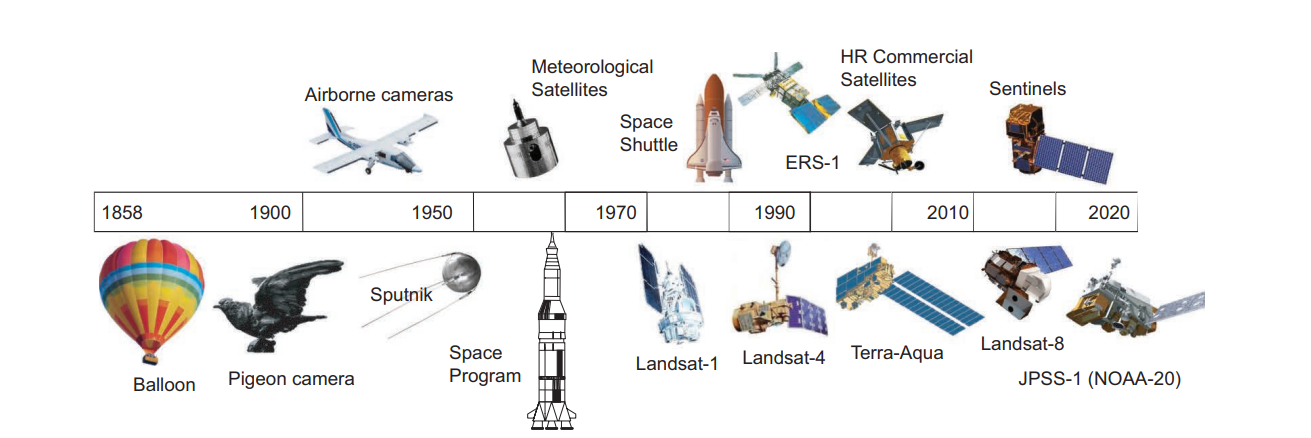
\includegraphics[width=\textwidth]{img/RS_timeline.png}
  \caption{Timeline of remote sensing platform development, from early airborne cameras to modern Earth observation satellites. Adapted from \cite{book_Satellite_RS}.}
  \label{fig:RS_timeline}
\end{figure}


\section{Copernicus: Europe's eyes on Earth}
Copernicus, known as the most ambitious Earth observation programme, is the Earth observation component of the European Union's Space Programme.
It is funded, coordinated, and managed by the European Commission in cooperation with partners such as the European Space Agency (ESA) and the European Organisation for the Exploitation of Meteorological Satellites (EUMETSAT)\footnote{https://www.eumetsat.int/}. The programme was named after the European scientist and observer Nicolaus Copernicus\footnote{https://www.biography.com/scientists/nicolaus-copernicus}. It integrates satellite and in situ observations (e.g., ground stations, airborne and seaborne instruments) to provide reliable, up-to-date information. Its services cover six domains: land, marine, atmosphere, emergency management, security, and climate change. 

The Copernicus Space Component features a new family of dedicated satellites,
called Sentinels, depicted in Figure \ref{fig:sentinels}, specifically designed for the operational needs of the Copernicus programme. 

\begin{figure}[H]
  \centering
  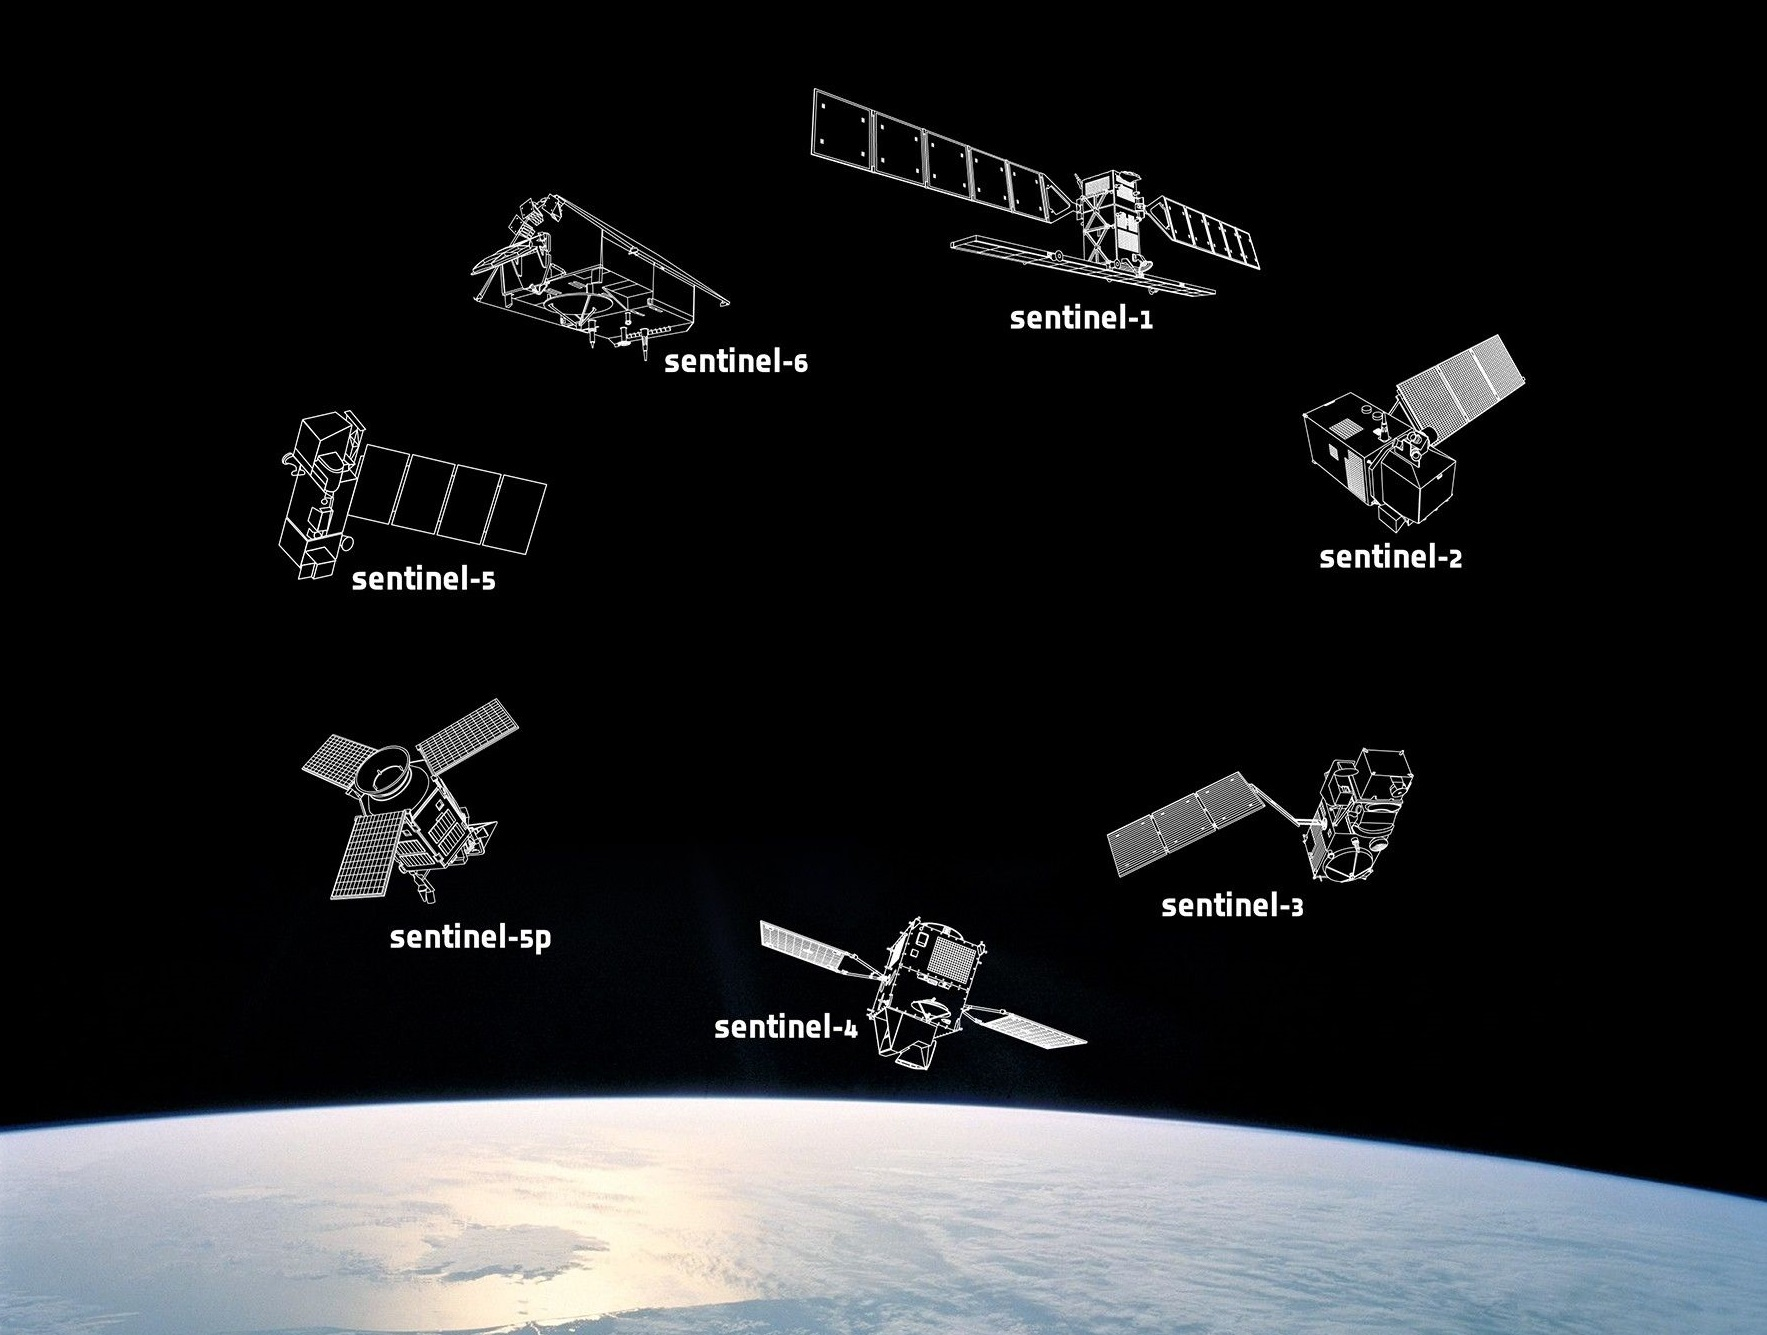
\includegraphics[width=0.95\textwidth]{img/sentinels.png}
  \caption{An artist's impression of the Copernicus Sentinel Missions. Source: ESA.}
  \label{fig:sentinels}
\end{figure}

On 3 April 2014, the deployment of the Copernicus Space Component began with the
launch of the \textsc{Sentinel-1} radar satellite, operating in the C-band and providing all-weather, day-and-night radar imagery. It was followed by its radar successors in 2016 and 2024. Its synthetic aperture radar (SAR) instruments are crucial for monitoring land deformation, subsidence, sea-ice dynamics, and emergency situations such as flooding and earthquakes \cite{ESA_Copernicus,ESA_SentinelMissions}.

\textsc{Sentinel-2}, launched in 2015, 2017, and 2024, is designed to deliver high-resolution, multispectral optical images, supporting applications such as agriculture, forestry, land use, disaster management, and climate studies. Its 13 spectral bands enable detailed analysis of vegetation health, water quality, and land cover dynamics \cite{ESA_Copernicus}.

The two \textsc{Sentinel-3} satellites, launched on 16 February 2016 and 25 April 2018, provide data for services relevant to the ocean and land. They carry instruments to measure sea surface topography, sea and land surface temperature, and ocean and land colour, providing essential data for oceanography, marine resource management, and climate monitoring \cite{ESA_SentinelMissions,ESA_Copernicus}.

\textsc{Sentinel-4} is an ultraviolet, visible, and near-infrared spectrometer carried on the Meteosat Third Generation Sounder satellites. Launched on 1 July 2025, it is dedicated to monitoring atmospheric composition and air quality over Europe and parts of North Africa. It provides hourly measurements of key trace gases and aerosols, enabling near-real-time assessments of air pollution, UV radiation, and climate-relevant processes \cite{ESA_Copernicus}.

Launched on 13 October 2017, the \textsc{Sentinel-5P} mission (Sentinel-5 Precursor) is the first Copernicus mission dedicated to monitoring the atmosphere. It provides high spatio-temporal resolution data for air quality, ozone and UV radiation, as well as climate monitoring and forecasting \cite{ESA_SentinelMissions}.

\textsc{Sentinel-6} is dedicated to high-precision ocean monitoring, focusing on sea surface topography. It continues the long-term record of satellite altimetry, measuring global sea level rise and ocean circulation patterns. These data are critical for climate change research, weather forecasting, and operational oceanography. Sentinel-6 was launched on 21 November 2020 \cite{ESA_SentinelMissions}. 

Looking into the future, six Sentinel Expansion missions will join the fleet. These include, among others, the Hyperspectral Imaging Mission, the Polar Ice and Snow Topography Altimeter, and the Anthropogenic Carbon Dioxide Monitoring mission \cite{ESA_Copernicus}.

Since the focus of this work is on SAR and Optical data, only Sentinel-1 and 2 will be discussed in details in the next sections. 
\subsection{Sentinel-1}
The following description is based on the official SentiWiki resource provided by the European Space Agency \cite{sentiwiki}. 

Sentinel-1, launched on 3 April 2014, constitutes the radar component of the European Copernicus Programme. The mission is designed as a constellation of two sun-synchronous, near-polar orbiting satellites in the same orbital plane, separated by 180° in phase. Equipped with C-band synthetic aperture radar (SAR) operating at 5.4~GHz, Sentinel-1 provides continuous, all-weather, day-and-night imaging capability. Sentinel-1A was followed by Sentinel-1B in 2016, which ceased operations after an anomaly in 2021 and was subsequently replaced by Sentinel-1C in 2024.  

The SAR instrument actively transmits microwave signals towards the Earth and records the backscattered response. Both amplitude and phase are preserved, enabling the reconstruction of high-resolution images. Polarisation diversity further enhances information extraction, as different surfaces exhibit characteristic scattering signatures, supporting classification and retrieval of geophysical parameters.  

Sentinel-1 operates in four exclusive acquisition modes: Stripmap (SM), Interferometric Wide Swath (IW), Extra-Wide Swath (EW), and Wave (WV). These modes achieve spatial resolutions down to 5~m and swath widths of up to 400~km. The system supports single (HH or VV) and dual (HH+HV or VV+VH) polarisation. While SM, IW, and EW modes allow a duty cycle of up to 30 minutes per orbit, WV mode extends this to 75 minutes. Over land, IW mode with VV+VH polarisation is the primary operational configuration, balancing revisit performance, service requirements, and the creation of a consistent long-term archive. For open-ocean observations, WV mode with VV polarisation is predominantly employed, while EW mode is mainly used for sea-ice monitoring and maritime surveillance in high-latitude regions. SM mode is activated only for small islands or in response to emergencies. Across all modes, products are provided at multiple processing levels, from raw SAR data (Level-0) to geophysical ocean products (Level-2 OCN).  

The revisit capabilities of Sentinel-1 are particularly notable. In IW mode, a single satellite can achieve global coverage every 12 days, while the two-satellite constellation reduces the repeat cycle to six days, completing 175 orbits per cycle. These systematic observations, combined with advanced interferometric capabilities, enable the precise detection of land subsidence, structural deformation, and ground movements that are otherwise imperceptible. Such data are invaluable for urban planning, geohazard monitoring, and applications in mining, geology, and risk assessment for infrastructure and natural hazards \cite{sentiwiki}.  

\subsection{Sentinel-2}
The following description is based on the official SentiWiki resource provided by the European Space Agency \cite{sentiwiki}. 

Sentinel-2 is the optical imaging mission of the Copernicus Programme, designed to provide systematic, high-resolution observations over land and coastal regions. The mission consists of a constellation of two sun-synchronous satellites in the same orbital plane, phased 180° apart, ensuring global coverage with a revisit frequency of five days at the Equator. Sentinel-2A was launched in 2015, followed by Sentinel-2B in 2017 and Sentinel-2C in September 2024, the latter ensuring mission continuity as Sentinel-2A approaches the end of its operational lifetime.  

Each satellite carries a single payload: the Multi-Spectral Instrument (MSI). This passive optical sensor collects sunlight reflected from the Earth’s surface, splitting the incoming radiation into two focal plane assemblies: one covering the visible and near-infrared (VNIR) and the other the shortwave infrared (SWIR). The instrument has a swath width of 290~km, which is considerably wider than comparable missions such as Landsat 5/7 (185~km) or SPOT-5 (120~km).  

The MSI samples 13 spectral bands at three spatial resolutions: four bands at 10~m (Blue, Green, Red, and Near-Infrared), six bands at 20~m (red-edge and SWIR), and three bands at 60~m (aerosol, water vapour, and cirrus). These bands span the VNIR to SWIR regions of the electromagnetic spectrum and are tailored to applications including vegetation and crop monitoring, land cover mapping, water quality assessment, snow and ice monitoring, cloud screening, and atmospheric correction. An overview of the spectral bands is provided in Table~\ref{tab:sentinel2_bands}.  

\begin{table}[h]
\centering
\caption{Sentinel-2 MSI spectral bands with central wavelength and spatial resolution \cite{sentiwiki}.}
\label{tab:sentinel2_bands}
\begin{tabular}{@{}lll@{}}
\toprule
\textbf{Band} & \textbf{Central Wavelength [nm]} & \textbf{Resolution [m]} \\ \midrule
B1  & 443  (Aerosols)                & 60 \\
B2  & 490  (Blue)                    & 10 \\
B3  & 560  (Green)                   & 10 \\
B4  & 665  (Red)                     & 10 \\
B5  & 705  (Red edge)                & 20 \\
B6  & 740  (Red edge)                & 20 \\
B7  & 783  (Red edge)                & 20 \\
B8  & 842  (NIR)                     & 10 \\
B8a & 865  (Red edge)                & 20 \\
B9  & 945  (Water vapour)            & 60 \\
B10 & 1375 (Cirrus)                  & 60 \\
B11 & 1610 (SWIR)                    & 20 \\
B12 & 2190 (SWIR)                    & 20 \\ \bottomrule
\end{tabular}
\end{table}

Sentinel-2 imagery is systematically and freely available, supporting several Copernicus services. The Copernicus Land Monitoring Service (CLMS) employs Sentinel-2 for land cover and forest mapping, crop monitoring, ecosystem assessment, and climate change adaptation. The Copernicus Marine Environment Monitoring Service (CMEMS) relies on Sentinel-2 to derive products such as turbidity, chlorophyll, suspended particulate matter, bathymetry, and ice analysis. The Copernicus Emergency Management Service (CEMS) uses Sentinel-2 extensively in disaster response, particularly for rapid mapping of floods, fires, and earthquakes. By enabling systematic, frequent, and global observations, Sentinel-2 has become a cornerstone of Copernicus services, supporting environmental monitoring, resource management, and disaster response worldwide \cite{sentiwiki}.  

Together, Sentinel-1 and Sentinel-2 provide complementary SAR and optical observations, which form the basis of this thesis aiming to translate SAR imagery into its optical counterpart.

\section{Cloud Removal}
As briefly mentioned in the sections above, optical remote sensing imagery, such as Sentinel-2 products, represents a key source of Earth observation data. Compared to SAR observations, multispectral images contain rich spectral information and are readily interpretable by the human eye. Such data play an essential role in a wide range of applications, including environmental monitoring, resource exploration, and disaster assessment. While the quality and quantity of satellite observations have dramatically increased in recent years, one common problem persists for optical remote sensing imagery: \textbf{cloud cover}.

Based on findings from the International Satellite Cloud Climatology Project (ISCCP), average global cloud cover surpasses 66\% \cite{dl_cloud_detection_survey,aCGAN_fuse_sar_MS,CR_SEN2_dRNN}, with 55\% over land surface alone \cite{CR_SEN2_dRNN}, preventing optical satellites from acquiring valuable information about the Earth's surface due to the frequent presence of clouds in the imagery. In contrast to SAR instruments, optical sensors cannot penetrate clouds, resulting in considerable data gaps in both the spatial and temporal domains. For applications requiring consistent time series, e.g., agricultural monitoring, or where a specific scene must be observed at a given time, e.g., disaster monitoring, cloud cover represents a serious limitation \cite{CR_SEN2_dRNN}. The diversity of clouds —including thin and thick clouds as well as haze— together with the wide range of occlusion scenarios and their uneven distribution, poses an additional challenge for image reconstruction and the generalizability of cloud removal techniques\cite{CR_Advances_Review_ORS}.

Consequently, removing clouds and obtaining cloud-free optical data to retrieve surface information is both of theoretical importance and practical necessity. Cloud removal in optical remote sensing imagery aims to mitigate or eliminate the influence of clouds, thereby revealing more accurate and complete surface details \cite{CR_Advances_Review_ORS}. In response to this challenge, a wide range of approaches have been proposed. These methods can broadly be divided into three categories: (i) single-image methods, (ii) multimodal-based methods, and (iii) multitemporal-based methods \cite{CR_Advances_Review_ORS}. The main categories and their characteristics are summarized below

\begin{enumerate}[label=(\Alph*)]
    \item \textbf{Single-image methods:} Constrained by the limited acquisition capabilities of early remote sensing data, single-image cloud removal techniques attempt to restore surface information using only the cloudy optical image. Classical approaches employ statistical and physical models such as spatial similarity, frequency filtering, or atmospheric scattering models (e.g., the dark channel prior). With the advent of deep learning, CNNs, U-Nets, and GAN-based architectures have been applied to learn the mapping from cloudy to cloud-free domains, sometimes extended with unpaired learning schemes like CycleGANs. While these methods demonstrate effectiveness for thin or semi-transparent clouds, their reliance on information present in a single image limits their applicability to dense cloud cover. In such cases, they cannot reliably reconstruct surface features, which has motivated the integration of external data sources such as SAR imagery.
    
    \item \textbf{Multimodal-based methods:} Multimodal strategies explicitly integrate auxiliary data from other sensors to improve optical image restoration. Multispectral-based methods exploit the differential sensitivity of spectral bands, but the most notable progress has been achieved by fusing synthetic aperture radar (SAR) with optical imagery. SAR-to-optical image translation has emerged as a powerful paradigm in this context, as SAR penetrates cloud layers and provides structural information that can guide optical reconstruction. A wide range of approaches have been proposed, including CNN-based fusion, conditional GANs (cGANs), and CycleGAN-style frameworks, which either translate SAR features into optical-like imagery or combine them with partially corrupted optical inputs. These methods have proven especially effective in recovering surface information under dense and persistent cloud conditions, although challenges remain in terms of data registration, modality differences, and SAR-induced speckle noise.
    
    \item \textbf{Multitemporal-based methods:} Multitemporal approaches leverage repeated acquisitions of the same location at different times to fill in cloud-covered areas. Non-blind methods use cloud masks to guide restoration, whereas blind methods directly infer cloud-free information from temporal sequences. Techniques range from traditional model-driven approaches, such as low-rank tensor decomposition and sparse representation, to data-driven deep learning frameworks that learn spatio-temporal mappings. Recent research has also begun to combine multitemporal optical data with SAR, creating hybrid SAR–optical time series methods that enhance robustness under persistent cloud cover and enable more accurate SAR-to-optical translation. Although highly effective for dense cloud removal, these approaches face challenges such as geometric misalignment, temporal variability in land cover, and the need for large, paired training datasets.
\end{enumerate}

As shown in Table~\ref{tab:cloud_removal_categories}, research on cloud removal has been uneven across categories. Single-image methods have been the most extensively studied due to their simplicity and minimal data requirements, though their effectiveness is limited under dense clouds. Multimodal approaches, particularly SAR–optical fusion, have gained significant traction in recent years and are currently the most active research direction. By contrast, multitemporal methods, while highly effective in principle, are less frequently explored because of the challenges in acquiring consistent, well-aligned time series data.

\begin{table}[ht]
\centering
\caption{Summary of cloud removal categories, their advantages and limitations \cite{CR_Advances_Review_ORS, sar_2_opt_CGAN_survey_taxonomy}.}
\label{tab:cloud_removal_categories}
\begin{adjustbox}{max width=\textwidth, keepaspectratio=false}
\begin{tabular}{p{2.5cm} p{6cm} p{6cm} p{3cm}}
\toprule
\textbf{Category} & \textbf{Advantages} & \textbf{Limitations} & \textbf{Representative literature} \\
\midrule
\textbf{Single-image} & 
\begin{itemize}[nosep,leftmargin=*]
  \item No auxiliary data required (cost- and time-efficient).
  \item Effective for thin or semi-transparent clouds.
  \item Straightforward implementation with statistical/physical models or deep learning.
\end{itemize} &
\begin{itemize}[nosep,leftmargin=*]
  \item Ineffective for dense or opaque clouds.
  \item Often introduces artifacts or color distortions.
  \item Deep learning requires large paired datasets, which are difficult to obtain.
\end{itemize} &
\cite{single_variation} \cite{single_haze_removal_dark_prior} \cite{single_artifact_free_CR_GAN} \cite{single_thin_CR_ORS_GAN_phys} \cite{single_multi_DR_CR} \cite{single_CR_DLM_matting} \cite{single_AGLC_GAN} \cite{single_PNBT_CR} \cite{single_CGAN_scattering_martian} \\
\midrule
\textbf{Multimodal} &
\begin{itemize}[nosep,leftmargin=*]
  \item Integrates complementary information from other sensors.
  \item Multispectral bands provide spectral redundancy.
  \item SAR–optical fusion enables SAR-to-optical translation, penetrating cloud layers.
  \item Suitable for both thin and thick clouds.
\end{itemize} &
\begin{itemize}[nosep,leftmargin=*]
  \item Requires accurate registration of heterogeneous data.
  \item SAR data introduces speckle noise.
  \item High computational complexity and preprocessing effort.
\end{itemize} &
\cite{A_cGAN_fuse_sar_MS_CR} \cite{sar2opt_cGAN_Optim_oppr_limits} \cite{syn_ms_sar_opt_MT_cGAN} \cite{CR_SEN2_dRNN} \cite{GAN_gen_synt_MS} \cite{s2o_ViT_cGAN} \cite{CR_RS_GAN_s2o} \cite{s2o_Thermodynamics} \cite{c_diffusion_s2o} \cite{s2o_color_super_diff} \cite{S2MS_GAN} \cite{SAR_DeCR} \\
\midrule
\textbf{Multitemporal} &
\begin{itemize}[nosep,leftmargin=*]
  \item Exploits temporal redundancy to reconstruct cloudy regions.
  \item Effective for dense and extensive cloud cover.
  \item Deep learning models can capture spatio-temporal correlations.
  \item Can be extended with SAR–optical time series for improved robustness.
\end{itemize} &
\begin{itemize}[nosep,leftmargin=*]
  \item Sensitive to geometric misalignment and temporal variability.
  \item Requires consistent multitemporal datasets, which may be unavailable.
  \item Landscape or seasonal changes reduce restoration accuracy.
\end{itemize} &
\cite{syn_ms_sar_opt_MT_cGAN} \cite{CR_RS_spati_atten_GAN} \cite{UnCRtainTS} \cite{assessing_MT_cGANS_s2o_crop} \cite{DiffCR} \\
\bottomrule
\end{tabular}
\end{adjustbox}
\end{table}

In summary, cloud removal research spans single-image, multimodal, and multitemporal strategies, each with distinct advantages and limitations, as outlined in Table~\ref{tab:cloud_removal_categories} together with representative literature. Among these, SAR-to-optical image translation has recently emerged as a particularly promising direction, as it leverages the cloud-penetrating capability of SAR while producing optical-like imagery suitable for interpretation and analysis. This thesis builds on this line of research by systematically investigating and advancing SAR-to-optical translation methods for cloud removal.

\section{Generative AI}
\subsection{Pre-GenAI: Classical Approaches}
\subsection{Deep Learning and Computer Vision}
\subsection{Generative Adversarial Networks (GANs)}
\subsection{Diffusion Models}
\subsection{Vision Transformer}
\subsection{Vision Mamba}

\section{Application and Relevance to KIWA}


